% MIDL 2027 paper (full-paper track, anonymous submission).
% MIDL/JMLR single-column template (https://github.com/MIDL-Conference/MIDLLatexTemplate).
% Numbers from outputs/reports/OFFICIAL_W_FREEZE.txt, camelyon_cross_seed_w.txt,
% camelyon_coverage_val_split.txt, pathology_risk_coverage/coverage_bootstrap_ci.txt.
% Official Kendall W is never recomputed here.
\documentclass[anon]{midl}

\jmlrvolume{-- Under Review}
\jmlryear{2027}
\jmlrworkshop{Full Paper -- MIDL 2027 submission}
\editors{Under Review for MIDL 2027}

\usepackage{booktabs}
\newcommand{\etal}{et al.}

\title{Detector Ranking is Not Architecture-Invariant under Medical Covariate Shift}

\midlauthor{\Name{Anonymous Author(s)} \Email{anonymous@example.edu}\\
\addr Affiliation withheld for review}

\begin{document}
\maketitle

\begin{abstract}
Post-hoc out-of-distribution (OOD) detectors are almost always ranked on a single backbone.
We ask how much that ranking moves when only the backbone changes, holding one medical covariate split fixed.
On Camelyon17 hospital-2 (WILDS), Kendall's $W=0.694$ across eight CNN families and seven scores (seed~42); MSP AUROC spans $0.515$ (ResNet-50) to $0.883$ (DenseNet-121), and the DenseNet MSP jump holds on $5/5$ seeds.
But retraining one fixed architecture with a different seed reorders the seven scores almost as much: cross-seed $W$ is $0.600$--$0.931$ (mean $0.780$), so the full-ranking reorder cannot be attributed to architecture alone.
\textbf{What is stable is the feature-space family}: Mahalanobis or $k$NN is rank~1 on every backbone and every seed tested.
Skin ISIC$\to$PAD does not reproduce the MSP jump ($W=0.791$).
AUROC is not a proxy for deployment coverage: the sign of the AUROC versus coverage@risk\,$10\%$ disagreement flips between Camelyon and MIDOG, and on a patient-disjoint split of hospital~2, choosing the backbone by validation coverage@risk instead of validation AUROC raises held-out coverage from $0.539$ to $0.754$.
A pre-registered ViT-B/16 MSP of $0.884$ met a locked threshold of $0.6947$.
The protocol: default to feature-space scores, do not copy a logit-score ranking across backbones or seeds, and pick a triage backbone from coverage@risk on a target-domain validation split, not from an AUROC table.
\end{abstract}

\begin{keywords}
out-of-distribution detection, domain shift, histopathology, dermoscopy, benchmark evaluation, model selection
\end{keywords}

\section{Introduction}

\begin{figure}[t]
\floatconts
  {fig:msp}
  {\caption{\textbf{The claim in one figure.}
  (a)~Same Camelyon hospital-2 split, same seven scores: switching ResNet-50$\to$DenseNet-121 lifts logit AUROC by ${\sim}0.37$ while Mahalanobis and $k$NN stay on top.
  (b)~On the full labeled test set (retrospective), the AUROC-highest backbone (DenseNet) has coverage@risk\,$10\%=0.078$ while the coverage@risk-highest backbone (MobileNet) reaches $0.904$: AUROC rank and coverage rank disagree. \sectionref{sec:coverage} gives the held-out version.}}
  {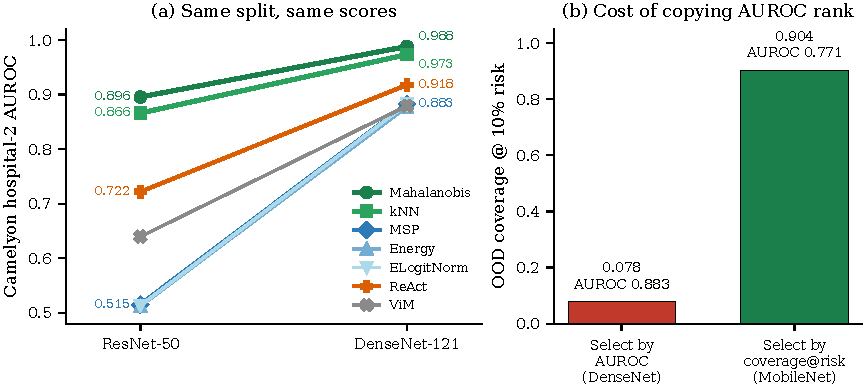
\includegraphics[width=\linewidth]{fig/fig1_hook.pdf}}
\end{figure}

We test one hypothesis: \emph{under a fixed medical covariate shift, post-hoc detector ranking is an architecture property}.
On Camelyon17 hospital-2, ResNet-50 MSP AUROC is $0.515$ while DenseNet-121 is $0.883$ (\figureref{fig:msp}a).
A lab that copies an OpenMIBOOD-style ResNet-50 recipe and a lab that uses DenseNet are not ranking the same detectors.
And AUROC order does not predict coverage@risk order, so an AUROC table is not a safe guide to triage: on a patient-disjoint split, selecting by AUROC instead of coverage@risk loses $0.215$ held-out coverage at a $10\%$ risk budget (\figureref{fig:msp}b shows the retrospective full-test-set version).
The answer we reach is narrower than the hypothesis: retraining one architecture with a new seed reorders the scores about as much as changing the architecture, and only the feature-space scores are stable across both.

That hypothesis is \emph{not} that ranking was previously assumed architecture-invariant.
On natural-image semantic OOD, ranking already moves with architecture~\cite{zhang2023openoodv15,szyc2023uai,datko2026eswa,claros2025arxiv}.
OpenMIBOOD~\cite{openmibood2025} already showed that ImageNet method ranking does not transfer to medical data and that feature-space scores outperform logit scores under a frozen classifier per domain.
The orthogonal question is: \textbf{holding one medical covariate-shift dataset fixed, how much does ranking move when only the backbone changes?}

The rest of the paper is that test, in order.
Camelyon discovers the shift: Kendall $W=0.694$ and a backbone-dependent MSP jump.
Five seeds verify the DenseNet MSP jump ($5/5$), and a cross-seed $W$ bounds how much of the ranking reorder is training noise.
Matched-recipe training asks whether that jump is architecture or optimizer.
Skin falsifies a universal MSP-jump law, while feature ranks stay 1--2.
MIDOG is the deployment readout: the \emph{sign} of AUROC versus coverage@risk disagreement flips.
A pre-registered ViT-B/16 tests whether the Camelyon MSP jump extends past CNNs.
The contribution is a protocol, not a detector.

\paragraph{Contributions.}
\begin{enumerate}
\item \textbf{On Camelyon, logit scores reorder across backbones---and across seeds.}
Official Kendall $W=0.694$ ($n{=}8$, 7 methods, seed~42).
MSP AUROC span $0.515$--$0.883$ matches the Maha${-}$MSP gap on ResNet-50.
Copying ResNet-50's winning logit (ReAct) onto ConvNeXt costs $0.185$ AUROC.
The seed-robust MSP jump is DenseNet-121 ($0.265{\pm}0.065$, $5/5$); ConvNeXt and EffV2-S@224 are $4/5$, MobileNet/RegNet $3/5$, EffB3 $2/5$.
Cross-seed $W$ at fixed architecture is $0.600$--$0.931$, so the full-ranking reorder is not architecture alone; feature-space scores hold rank~1 in all $20$ anchor${\times}$seed cells.
\item \textbf{Skin falsifies universality.}
ISIC$\to$PAD ($n{=}8$, $W{=}0.791$): Maha rank-1 and $k$NN rank-2 on all eight; MSP stays in a narrow band. Not a second Camelyon jump.
\item \textbf{AUROC is not a reliable proxy for deployment coverage.}
The sign of the AUROC versus coverage@risk\,$10\%$ disagreement flips between Camelyon and MIDOG~\cite{geifman2019selectivenet,traub2024augrc}.
On a patient-disjoint split of Camelyon hospital~2, selecting by validation coverage@risk instead of validation AUROC raises held-out coverage from $0.539$ to $0.754$ (\sectionref{sec:coverage}); the larger full-test-set gap ($0.826$) is retrospective only.
\item \textbf{A locked prediction.}
Before training: ViT-B/16 Camelyon MSP ${\ge}0.6947$. Observed $0.884$. Held out of the 8-CNN $W$.
\end{enumerate}

\section{Related work}

\begin{table}[t]
\floatconts
  {tab:related}
  {\caption{Closest ranking-vs-backbone papers. Architecture-sensitive ranking exists on natural-image semantic OOD; the increment here is a held-fixed medical covariate split, zoo-scale $W$, and operational coverage.}}
  {\small
  \begin{tabular}{@{}lcccc@{}}
  \toprule
  Work & \#arch. & Shift & Rank stat. & Utility \\
  \midrule
  OpenOOD v1~\cite{yang2022openood} & 1/set & semantic & --- & AUROC \\
  OpenOOD v1.5~\cite{zhang2023openoodv15} & 3 & semantic & qualitative & AUROC \\
  Szyc \etal~\cite{szyc2023uai} & 3 var. & CIFAR sem. & rank $\Delta$ & AUROC \\
  Datko \etal~\cite{datko2026eswa} & per line & natural & claimed stable & AUROC \\
  OpenMIBOOD~\cite{openmibood2025} & 1/domain & medical & --- & AUROC \\
  \textbf{Ours} & \textbf{8+ViT} & \textbf{covar.} & \textbf{Kendall $W$} & \textbf{AUROC+cov.} \\
  \bottomrule
  \end{tabular}}
\end{table}

OpenMIBOOD~\cite{openmibood2025} ranks 24 post-hoc detectors with a \textbf{single frozen classifier per medical domain}.
It shows that ImageNet method ranking does not transfer to medical data and that feature-space scores outperform logit scores under that protocol.
\tableref{tab:related} locates the increment: we hold the dataset fixed and change the backbone.

OpenOOD v1~\cite{yang2022openood} fixes architecture on purpose.
OpenOOD v1.5~\cite{zhang2023openoodv15} compares three ImageNet models on semantic near/far OOD and reports that ``different post-processor may favor different architecture,'' without Kendall's $W$ and without a covariate hospital split.
Szyc \etal~\cite{szyc2023uai} show rankings change across three ResNet CIFAR implementation variants.
Datko \etal~\cite{datko2026eswa} claim an architecture-specific winner that transfers across natural-image OOD---the opposite of a single-split concordance statistic.\footnote{This citation could not be independently verified against a primary source at the time of writing; see \texttt{refs.bib}. Confirm the original DOI/URL before submission.}
Claros Olivares and Brockmeier~\cite{claros2025arxiv} rank confidence scores with AURC/AUGRC on CIFAR / TinyImageNet; they do not report a sign-flip of AUROC versus coverage@risk\,$10\%$ across medical covariate domains.

OoD-Bench~\cite{ye2022oodbench} is OOD generalization, not detection.
WILDS~\cite{koh2021wilds} supplies Camelyon17 and iWildCam; iWildCam is a negative bound, not a third main domain.

\section{Setup}

\subsection{Shifts}

Camelyon17~\cite{bandi2019camelyon17}, via the WILDS~\cite{koh2021wilds} split: hospitals 0, 3, 4 as ID and hospital~2 as OOD (WILDS's official OOD-test domain); founding cell, official $W$, $n{=}8$.
Hospital~1 is WILDS's official OOD-\emph{validation} domain; we do not use it for any number in the main paper and report it only in the held-out stain-jitter check (\appendixref{app:suppl}).
Skin ISIC$\to$PAD~\cite{codella2019isic2018,pacheco2020pad}: feature rank-stability without an MSP jump.
MIDOG~\cite{aubreville2023midog}: OpenMIBOOD's~\cite{openmibood2025} 1a vs.\ 1b{+}1c split and checkpoints, coverage sign-flip; official $W$ is $n{=}3$.
We build on OpenMIBOOD's public MIDOG split and ResNet-50 checkpoint as an external reference.
Public R50 AUROC ${\sim}0.59$ is \emph{theirs}; in-house R50 MSP $0.512$ is \emph{ours}. We never mix the two.

\subsection{Backbones}

Eight CNN-family models, ImageNet initialization, 10-epoch fine-tune, seed~42, train-frac $1.0$ on Camelyon: ResNet-18/50~\cite{he2016resnet}, DenseNet-121~\cite{huang2017densenet}, ConvNeXt-Tiny~\cite{liu2022convnext}, MobileNetV3-Large~\cite{howard2019mobilenetv3}, RegNetY-3.2GF~\cite{radosavovic2020regnet}, EfficientNet-B3~\cite{tan2019efficientnet} at native 300, and EfficientNetV2-S~\cite{tan2021efficientnetv2} at \textbf{224} (native 384 dropped).
Standard fine-tune recipes (Adam / AdamW / SGD) follow each family's common practice and are \emph{not} forced-identical Adam.
That confound is measured in \sectionref{sec:m1m2}.
Only resolution was isolated in a controlled pair (EffB3 @224 vs.\ @300; EffV2-S @224 vs.\ @384).
ViT-B/16~\cite{dosovitskiy2021vit} @224 is held out of $W$.

\subsection{Scores and statistics}

Seven post-hoc scores: MSP~\cite{hendrycks2017baseline}, Energy~\cite{liu2020energy}, energy of logit-normed logits (ELogitNorm), ViM~\cite{wang2022vim}, ReAct~\cite{sun2021react}, Mahalanobis with Ledoit--Wolf covariance~\cite{lee2018mahalanobis,ledoit2004well}, and $k$NN~\cite{sun2022knn}.
Primary concordance: \textbf{Kendall's $W$ per domain, never pooled}.
Jump: $\mathrm{MSP}-\mathrm{mean}(\mathrm{R18},\mathrm{R50})\ge 0.15$.
Feature drag: Maha or $k$NN on a new backbone below $\mathrm{median}(\mathrm{R18},\mathrm{R50},\mathrm{EffB3})-0.10$.
Official Camelyon ResNet mean MSP ${=}0.544654$; jump iff MSP ${\ge}0.695$ on that split.

Coverage@risk\,$10\%$ is OOD-triage: rank OOD samples by MSP (higher ${=}$ more ID-like) and take the largest coverage whose classifier risk is ${\le}10\%$.
ID-selective Camelyon is vacuous (ID-val acc ${\approx}99.5\%$) and is not cited.
AUROC and coverage@risk measure different things: AUROC is ID-vs-OOD separability of the detector score alone, while coverage@risk\,$10\%$ depends jointly on that ranking \emph{and} the classifier's own accuracy on the OOD domain, so the two need not agree, and a disagreement between them is not itself surprising without separately checking which one moved.
A comparison of the two on the full labeled OOD test set is retrospective; \sectionref{sec:coverage} therefore also selects on a patient-disjoint validation half and evaluates on the other half.

We tested whether the Camelyon MSP pattern is an artifact of input resolution, temperature scaling~\cite{guo2017calibration}, ID-only detector \emph{selection}, a CE{+}SupCon recipe~\cite{khosla2020supcon}, or train-time HED stain jitter.
None is a clean account (\sectionref{sec:failed} and \appendixref{app:suppl}).

\section{Results}

\subsection{Camelyon-17 discovers the ranking shift}
\label{sec:camelyon}

Official Kendall $W=\mathbf{0.694}$ ($n{=}8$, 7 methods).
This is the only Camelyon number called ``official $W$.''
Leave-one-backbone recomputation of $W$ ranges $0.676$--$0.738$; that is \emph{structural} sensitivity of the concordance statistic, not a $95\%$ CI (\appendixref{app:suppl}).

\begin{table}[t]
\floatconts
  {tab:cam}
  {\caption{Camelyon hospital-2 AUROC, \textbf{seed~42} (official $W$).
  Jump iff MSP ${\ge}0.6947$ vs.\ frozen ResNet mean $0.544654$.
  MSP range is ResNet-50${\to}$DenseNet.}}
  {\small
  \begin{tabular}{@{}lccccc@{}}
  \toprule
  Backbone & input & Maha (rank) & $k$NN (rank) & MSP & seed-42 jump \\
  \midrule
  ResNet-18 & 224 & 0.956 (1) & 0.936 (2) & 0.574 & no \\
  ResNet-50 & 224 & 0.896 (1) & 0.866 (2) & 0.515 & no \\
  DenseNet-121 & 224 & 0.988 (1) & 0.973 (2) & 0.883 & yes \\
  ConvNeXt-Tiny & 224 & 0.928 (1) & 0.916 (2) & 0.846 & yes \\
  MobileNetV3-L & 224 & 0.870 (2) & 0.904 (1) & 0.771 & yes \\
  RegNetY-3.2GF & 224 & 0.964 (1) & 0.956 (2) & 0.784 & yes \\
  EfficientNet-B3 & 300 & 0.885 (2) & 0.934 (1) & 0.803 & yes \\
  EfficientNetV2-S & \textbf{224} & 0.880 (1) & 0.856 (2) & 0.778 & yes \\
  \bottomrule
  \end{tabular}}
\end{table}

Feature methods occupy ranks 1--2 on every official backbone (Maha \#1 on $6/8$; $k$NN \#1 on EffB3 and MobileNet).
No backbone drags Maha/$k$NN past the $0.10$ feature-drag threshold.
On \tableref{tab:cam}, MSP spans $0.515$--$0.883$; Maha $0.870$--$0.988$; $k$NN $0.856$--$0.973$.
Incomplete concordance ($W{=}0.694$) is the logit ranks moving (\figureref{fig:ranks}).

\begin{table}[t]
\floatconts
  {tab:seeds}
  {\caption{Same eight Camelyon hospital-2 MSP cells on all five seeds $\{42,43,44,45,46\}$.
  Jump ${=}$ MSP minus that seed's ResNet mean; bar $0.15$.
  The last column is how many of those five seeds clear the bar.
  Official $W$ is seed~42 only.}}
  {\footnotesize
  \begin{tabular}{@{}lccccccl@{}}
  \toprule
  Backbone & 42 & 43 & 44 & 45 & 46 & jump mean${\pm}$sd & ${\ge}0.15$ \\
  \midrule
  ResNet-18 & 0.574 & 0.712 & 0.601 & 0.524 & 0.581 & --- & --- \\
  ResNet-50 & 0.515 & 0.621 & 0.619 & 0.515 & 0.661 & --- & --- \\
  ResNet mean & 0.545 & 0.667 & 0.610 & 0.520 & 0.621 & --- & --- \\
  DenseNet-121 & 0.883 & 0.865 & 0.868 & 0.845 & 0.826 & $0.265{\pm}0.065$ & $5/5$ \\
  ConvNeXt-Tiny & 0.846 & 0.799 & 0.803 & 0.764 & 0.785 & $0.207{\pm}0.067$ & $4/5$ \\
  MobileNetV3-L & 0.771 & 0.728 & 0.815 & 0.780 & 0.745 & $0.175{\pm}0.081$ & $3/5$ \\
  RegNetY-3.2GF & 0.784 & 0.778 & 0.836 & 0.830 & 0.724 & $0.198{\pm}0.089$ & $3/5$ \\
  EfficientNet-B3 & 0.803 & 0.731 & 0.643 & 0.818 & 0.678 & $0.142{\pm}0.125$ & $2/5$ \\
  EfficientNetV2-S@224 & 0.778 & 0.744 & 0.808 & 0.846 & 0.835 & $0.210{\pm}0.089$ & $4/5$ \\
  \bottomrule
  \end{tabular}}
\end{table}

\tableref{tab:seeds} reports the full five-seed MSP matrix: seeds verify the DenseNet MSP jump.
DenseNet-121 is the confirmed seed-robust jump ($5/5$).
ConvNeXt-Tiny and EfficientNetV2-S@224 are not seed-42 flukes ($4/5$) and are not promoted to $5/5$.
MobileNetV3 and RegNetY are $3/5$; EfficientNet-B3 is $2/5$ (its seed-42 jump $+0.258$ is a favorable draw relative to $0.142{\pm}0.125$).
The seed-42 matrix still shows a jump without feature drag.
The claim is narrower than ``$6/6$ non-ResNet, confirmed.''

Copying a logit ranking is not free.
ResNet-50's best logit is ReAct ($0.722$); on ConvNeXt the same score is $0.692$ against Energy $0.877$---a $0.185$ AUROC transfer cost.
Feature-space transfer regret is ${\le}0.05$ because Maha/$k$NN stay in ranks 1--2.

\paragraph{Cross-seed control.}
Is the incomplete concordance an architecture effect or training noise?
For the four anchors trained on all five seeds we compute Kendall's $W$ over the seven scores with the seeds, not the backbones, as raters.
Cross-seed $W$ is $0.931$ (ResNet-50), $0.800$ (ResNet-18), $0.789$ (DenseNet-121) and $0.600$ (EfficientNet-B3); mean $0.780{\pm}0.136$.
EfficientNet-B3's value is below the cross-architecture $0.694$, and cross-architecture $W$ over the same four anchors at a fixed seed is $0.750$--$0.915$.
Retraining one architecture therefore reorders the seven scores about as much as changing the architecture does, and the cross-architecture $W$ cannot be read as an architecture effect on its own.
What survives the control is narrower: a feature-space score is rank~1 in all $20$ anchor${\times}$seed cells (both in ranks 1--2 in $18/20$), and the DenseNet MSP jump ($5/5$ seeds) is an architecture effect on the MSP \emph{level}, not on the full ranking.
Backbone choice moves the logit leaderboard, but so does the seed; neither unseats the feature default.

\subsection{Skin falsifies a universal MSP jump}

Official $W=\mathbf{0.791}$ ($n{=}8$).
Maha is rank-1 and $k$NN rank-2 on \textbf{all eight} (\figureref{fig:ranks}).
MSP sits in a narrow band ($0.68$--$0.74$).
There is no Camelyon-style ResNet-vs-rest MSP jump.
EffV2-S@224 MSP is $0.737$; the native-384 cell that put $k$NN at rank~7 (MSP $0.823$) is a resolution artifact and is not in official $W$.
Skin is rank-stability of feature scores under a zoo: a replication of OpenMIBOOD's feature${>}$logit pattern \emph{across architectures}, not an MSP-jump.

\begin{figure}[t]
\floatconts
  {fig:ranks}
  {\caption{\textbf{Method rank by backbone} (1${=}$best AUROC).
  Feature-space scores occupy ranks 1--2 on every official backbone in both domains.
  Logit ranks move on Camelyon ($W{=}0.694$) and much less on skin ($W{=}0.791$), where Maha is rank-1 on $8/8$.}}
  {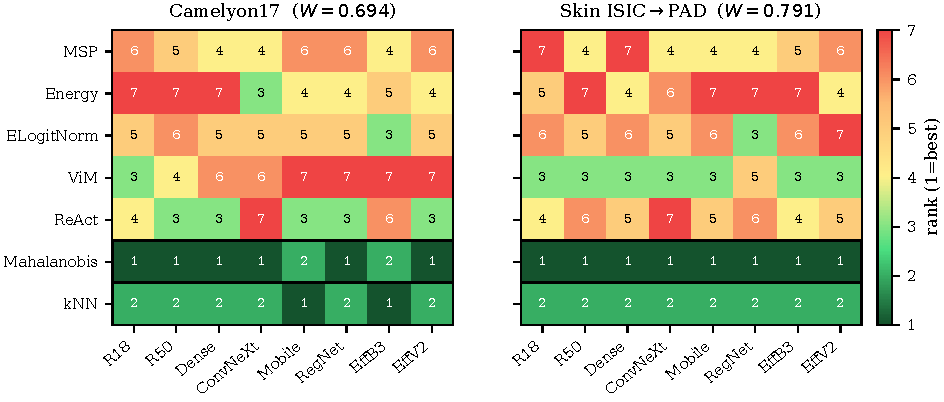
\includegraphics[width=\linewidth]{fig/fig2_rank_heatmaps.pdf}}
\end{figure}

\subsection{Optimizer challenges a clean architecture reading}
\label{sec:m1m2}

Resolution is not the Camelyon DenseNet / seed-42 pattern.
EffB3 Camelyon: $0.803$ @300 ${\to}$ $0.787$ @224 (the jump versus the official ResNet mean survives).
EffV2-S Camelyon: $0.726$ @384 ${\to}$ $\mathbf{0.778}$ @224 (the official cell; the jump is not a 384 artifact).
On skin, the EffV2-S @384 $k$NN collapse \emph{is} a resolution artifact and disappears at 224.
These two facts are not a slogan that ``resolution never matters.''

\paragraph{M1 --- jumpers trained with ResNet Adam}
($\mathrm{lr}{=}10^{-4}$, $\mathrm{wd}{=}10^{-4}$, batch $64$).
The four official zoo members whose standard recipe was not that Adam still jump versus the frozen official ResNet mean $0.545$:
ConvNeXt $0.820$ ($+0.275$), MobileNetV3 $0.737$ ($+0.193$), RegNet $0.805$ ($+0.261$), EffV2-S@224 $0.873$ ($+0.328$); all with id-val acc ${\ge}0.994$.
$4/4$ clean hits.
DenseNet and EffB3 already shared ResNet-Adam in the official zoo.
Recipe mismatch does \emph{not} explain the seed-42 jumps of those four members.
M1 is seed~42 only; the five-seed MSP matrix is \tableref{tab:seeds}.

\paragraph{M2 --- ResNets trained with ConvNeXt AdamW}
($\mathrm{wd}{=}0.05$).
ResNet-18 MSP $\mathbf{0.773}$ (enters the $0.695$ band; id-val $0.9957$).
ResNet-50 MSP $0.581$ (stays out; id-val $0.9958$).
ResNet \emph{can} jump under a non-default recipe.
Architecture is not a clean variable, independent of optimizer.
These two results point in opposite directions; we report both.

\subsection{ViT-B/16: a locked prediction}

Locked \emph{before} training, from the seed-42 zoo rule that non-ResNet-like cells jumped: MSP ${\ge}0.6947$.
Linear depth/parameter/receptive-field predictors are invalid on this $n{=}8$ and are not quoted.
Observed MSP $\mathbf{0.884}$, Maha $0.958$, $k$NN $0.941$.
The prediction holds.
Not a ninth $W$ column.

\subsection{Coverage@risk: the deployment cost}
\label{sec:coverage}

Protocol: OOD-triage coverage@risk\,$10\%$ with MSP, not ID-selective coverage.

On Camelyon hospital-2, the locked $n{=}4$ utility table has MSP AUROC order EffB3@300 ($0.803$) ${>}$ EffB3@224 ($0.787$) ${>}$ ResNet-18 ($0.574$) ${>}$ ResNet-50 ($0.515$), but coverage@risk\,$10\%$ order ResNet-50 ($0.149$) ${>}$ ResNet-18 ($0.145$) ${>}$ EffB3@300 ($0.107$) ${>}$ EffB3@224 ($0.013$).
The AUROC winner is not the coverage winner (\figureref{fig:cov}).

On MIDOG, official $n{=}3$ (in-house): MSP AUROC ResNet-50 $0.512$, EffB3 $0.486$, ResNet-18 $0.438$ (gaps are small).
Coverage@risk\,$10\%$: EffB3 $0.712$, ResNet-18 $0.442$, ResNet-50 $0.166$.
ResNet-50 is AUROC-highest and coverage-lowest.
The permutation is \emph{not} the Camelyon permutation.

\begin{figure}[t]
\floatconts
  {fig:cov}
  {\caption{\textbf{AUROC vs.\ coverage@risk\,$10\%$.}
  On Camelyon the AUROC-high EfficientNets have the \emph{lowest} triage coverage; on MIDOG the AUROC-high ResNet-50 is coverage-lowest.
  The sign of the disagreement flips.}}
  {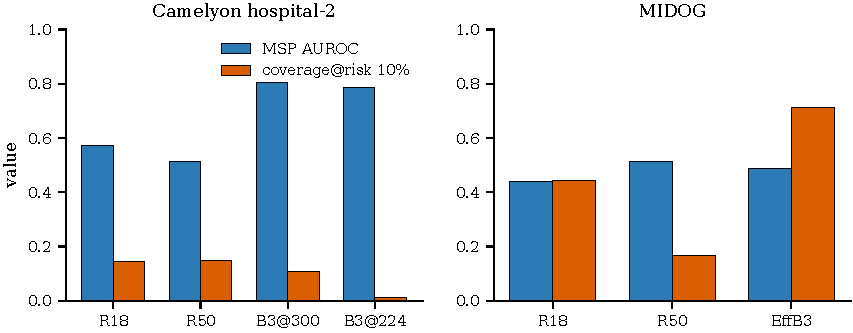
\includegraphics[width=0.92\linewidth]{fig/fig3_coverage_signflip.pdf}}
\end{figure}

AURC/AUGRC already assume that AUROC and coverage-based ranking can disagree~\cite{geifman2019selectivenet,traub2024augrc}.
The increment is the \emph{sign} of that disagreement flipping between two medical covariate domains under the same protocol, with no rule for which backbone wins.
On the full labeled Camelyon test set, AUROC order and coverage@risk order on the $n{=}8$ zoo diverge by $0.826$ coverage (DenseNet $0.078$ vs.\ MobileNet $0.904$; patch-bootstrap $95\%$ CI of the difference $[0.817, 0.837]$; \figureref{fig:msp}b).
That comparison is retrospective: it reads both rankings off the test labels, which do not exist at deployment time.

\paragraph{Held-out selection.}
To make it a procedure, we split the nine hospital-2 patients into two halves (stratified on the tumor label, grouped by patient, seed~42, frozen before any model was scored): six patients ($41{,}217$ patches) for selection, three ($43{,}837$) for evaluation.
Selecting the backbone with the highest validation MSP AUROC picks ConvNeXt ($0.877$), which reaches coverage@risk\,$10\%$ of $0.539$ on the test half.
Selecting by validation coverage@risk picks EfficientNetV2-S@224 ($0.821$), which reaches $0.754$: a $+0.215$ gain.
Both are well below the best test-half backbone (MobileNet, $1.000$), and coverage varies strongly with which patients fall in each half (one patient contributes $31{,}878$ patches, $85\%$ tumor).
Coverage-based selection on a target validation split helps, but at $n{=}8$ backbones and nine patients it is noisy, not solved.

\subsection{Frozen foundation models}

Camelyon linear-probe MSP does not invert: GigaPath~\cite{xu2024gigapath} $0.664$, Phikon~\cite{filiot2023phikon} $0.605$, UNI~\cite{chen2024uni} $0.599$, all ${>}0.5$.
MIDOG UNI / GigaPath MSP $0.445$ / $0.470$ is a MIDOG-only footnote.
FM Maha ${\sim}0.995$--$1.0$ is discussion support that feature${>}$logit can survive a training-paradigm change, not a pillar.

\section{Failed alternatives}
\label{sec:failed}

Each of the following was a precommitted test. None is hidden.

\textbf{Resolution} (from \sectionref{sec:m1m2}).
EffB3@224 MSP $0.787$; EffV2-S@224 MSP $0.778$.
Not a pixel-size explanation of \tableref{tab:cam}.

\textbf{Temperature $T^\ast$.}
Correlation of $T^\ast$ with the MSP jump: $r{=}0.268$, $p{=}0.52$.
DenseNet${-}$ResNet-18 MSP gap $0.308{\to}0.308$ after $T^\ast$.
Calibration/temperature is not the mechanism.

\textbf{ID-only Maha/MSP gate.}
Selecting a score from ID-only statistics is a \emph{selector}, not a detector.
On Camelyon it picks Maha on $2/8$ backbones; mean AUROC of the gated score $0.837$ versus always-Maha $0.940$.
The bar was matching Maha and ViM. It does not.

\textbf{CE{+}SupCon} ($\lambda{=}0.1$, $\tau{=}0.07$), ResNet-18 ${+}$ DenseNet.
Gap $0.308{\to}0.238$ ($23\%$; precommit bar was $50\%$ / ${\le}0.154$).
ResNet-18 MSP $0.574{\to}\mathbf{0.515}$ (worse; this is the SupCon cell, not official ResNet-50 MSP $0.515$).
Part of the shrink is the low model degrading.
Dirty; not a recipe.

HED stain jitter, an in-house MIDOG $n{=}8$ zoo, and a shift-type extract (covariate / task / far-OOD) are in \appendixref{app:suppl}.
Joint readout: no shift-type law, no stain mitigation, no Camelyon-style MSP jump on MIDOG.

\section{Discussion and limitations}

The hypothesis holds only in a narrow form, and fails as a cross-medical MSP-jump law.
On Camelyon, backbone choice changes the logit-score ranking and produces a seed-robust DenseNet MSP jump, but retraining one architecture reorders the seven scores about as much, so a cross-architecture Kendall's $W$ ($0.694$) is not by itself evidence of an architecture effect.
The stable finding is the feature-space family: Mahalanobis or $k$NN is rank~1 on every backbone and every seed we tested, when the shift looks like Camelyon \emph{and} when it does not (skin).
M1 preserves the seed-42 jumps under ResNet-Adam; M2 lets ResNet-18 enter the MSP band under ConvNeXt-AdamW: architecture is the dominant axis, not a clean one.
ViT-B/16 was a locked prediction, not a post-hoc ninth CNN.

The practical cost is not abstract.
Copying ResNet-50's logit winner onto ConvNeXt costs $0.185$ AUROC, and the cross-seed result implies a logit ranking does not reliably transfer even between seeds of one backbone.
Selecting a triage backbone from AUROC rather than from coverage@risk on a target validation split loses $0.215$ held-out coverage at a $10\%$ risk budget.
For benchmarks, this argues for reporting rank concordance across seeds as well as across backbones before reading a detector leaderboard, and for reporting coverage@risk on a held-out target split next to AUROC.

\paragraph{Limitations.}
(1)~\textbf{iWildCam bound.}
Locked 3-backbone cell: DenseNet MSP $0.575$ vs.\ ResNet mean $0.604$, jump $-0.029$.
Extra five CNNs vs.\ that domain's ResNet mean: ConvNeXt $0.601$, MobileNet $0.558$, RegNet $0.580$, EffB3 $0.577$, EffV2-S $0.650$; $0/5$ jump.
The Camelyon MSP-jump is absent on this non-medical covariate shift and may be biomedical-specific.
iWildCam is not pooled with Camelyon $W$.
(2)~\textbf{No clean mitigation.}
CE{+}SupCon is dirty (ResNet-18 MSP worse).
HED stain jitter is dirty (DenseNet MSP $0.780{<}0.80$).
The ID-only gate is a selector.
(3)~\textbf{MIDOG official $W$ is $n{=}3$} ($W{=}0.857$); the in-house $n{=}8$ zoo shows no MSP jump and does not replace it.
(4)~$W$ is per-domain; $0.694$ / $0.791$ / $0.857$ are not averaged.
(5)~No reader study: the operational claim stops at coverage@risk.
Patch-bootstrap $95\%$ CIs for Camelyon coverage are narrow (DenseNet $0.078$ $[0.067, 0.086]$, MobileNet $0.904$ $[0.898, 0.909]$) but ignore patient clustering; MIDOG ResNet-50 coverage $0.166$ $[0.004, 0.369]$ is wide.
(6)~Architecture is confounded with its standard recipe.
$5/5$ seed-robustness is DenseNet only.
Official $W$ stays seed~42.
Staining vs.\ scanner vs.\ tissue prep inside the hospital shift is not isolated.
(7)~\textbf{Held-out selection is one split of nine patients.}
The $+0.215$ gain comes from a single frozen patient split; repeated patient-level resampling was not run, and MIDOG ($n{=}3$) is not split.
(8)~\textbf{Seed variance is comparable to architecture variance in the full ranking.}
Cross-seed $W$ ($0.600$--$0.931$) covers four anchors on Camelyon only; it was not computed for skin or MIDOG.
Any claim about the full 7-score ranking, rather than about the feature-family default or the MSP level, is confounded with training seed.

Code for the architecture-zoo evaluation and coverage@risk will be released, crediting OpenMIBOOD for MIDOG imglists, the public ResNet-50 checkpoint, and the 1a / cs-ID / near-OOD protocol.

\section{Conclusion}

Under medical covariate shift, logit-based detector scores reorder with the backbone, but about as much with the training seed; the feature-space family stays on top across both.
On Camelyon that is a seed-robust DenseNet MSP jump, stable feature ranks, and a $0.215$ held-out coverage gain from selecting a backbone by validation coverage@risk instead of AUROC.
Skin keeps the feature ranks and drops the MSP jump.
MIDOG flips the sign of the AUROC--coverage disagreement.
A pre-registered ViT hit shows the Camelyon MSP jump is not a CNN-zoo accident; iWildCam does not reproduce it.
The protocol is the result: default to feature-space scores, do not copy a logit-score ranking across backbones or seeds, and estimate a backbone's coverage@risk on a held-out validation split of the deployment shift, not from an AUROC table.

\clearpage % references/appendix do not count toward the MIDL page limit

\bibliography{refs}

\appendix
\section{Supplementary material}
\label{app:suppl}

\paragraph{Leave-one-backbone $W$ is not a CI.}
Dropping one backbone and recomputing Camelyon $W$ on the remaining seven yields $0.676$--$0.738$ (largest increase when dropping ConvNeXt; largest decrease when dropping EffV2-S or RegNet).
This is structural sensitivity of the concordance statistic, not a seed confidence interval; the seed question is answered by the cross-seed control in \sectionref{sec:camelyon}.

\paragraph{HED stain jitter.}
Train-only HED stain jitter ($\sigma{=}0.20$, $p{=}1.0$) on ResNet-18, ResNet-50 and DenseNet-121, same Adam recipe as official, seed~42.
Precommit dirty-guard: DenseNet hospital-2 MSP ${<}0.80$ ${\Rightarrow}$ dirty.
Hospital-2 MSP: ResNet-18 $0.772$, ResNet-50 $0.593$, DenseNet $0.780$ (below $0.80$); gap DenseNet${-}$ResNet-18 $0.008$; id-val acc ${\ge}0.994$.
Held-out hospital-1 MSP: ResNet-18 $0.765$, ResNet-50 $0.685$, DenseNet $0.796$.
Dirty: part of the gap shrink is DenseNet falling ($0.883{\to}0.780$) while ResNet-18 rises. Not a mitigation.

\paragraph{MIDOG in-house zoo $n{=}8$ (not official $W$).}
Same 1a vs.\ 1b{+}1c protocol, not mixed with public OpenMIBOOD R50 ${\sim}0.59$.
MSP / Maha: ResNet-18 $0.438$ / $0.733$, ResNet-50 $0.512$ / $0.839$, DenseNet-121 $0.447$ / $0.910$, ConvNeXt-Tiny $0.521$ / $0.801$, MobileNetV3-L $0.469$ / $0.714$, RegNetY-3.2GF $0.553$ / $0.944$, EfficientNet-B3 $0.486$ / $0.673$, EfficientNetV2-S@224 $0.493$ / $0.581$.
MSP $0.44$--$0.55$ on all eight; $0/6$ non-ResNet jumps. A domain-scope bound, not a replacement of official $W$ ($n{=}3$, $0.857$).

\paragraph{Shift-type extract.}
Same eight Camelyon seed-42 classifiers, ID ${=}$ Camelyon \texttt{id\_val}.
Arm C (hospital-2, covariate): $6/6$ non-ResNet jumps. Arm T (MIDOG 1a, task shift): $0/6$. Arm F (CIFAR-10 test, far-OOD): $2/6$.
Per-arm Kendall $W$ (never pooled, not official): C $0.731$, T $0.692$, F $0.846$. No shift-type law.

\paragraph{Five-seed jumps.}
\figureref{fig:seedjumps} plots each backbone's MSP minus that seed's ResNet mean; the underlying MSP matrix is \tableref{tab:seeds}.

\begin{figure}[h]
\floatconts
  {fig:seedjumps}
  {\caption{Per-seed MSP jump versus that seed's ResNet mean. DenseNet stays above $0.15$ on all five seeds; EfficientNet-B3 does not.}}
  {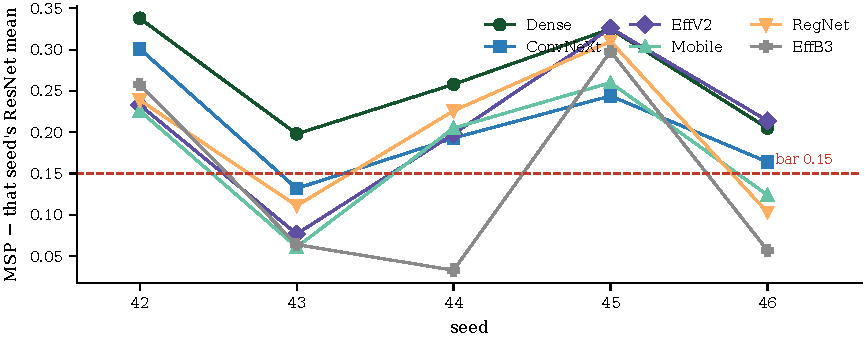
\includegraphics[width=0.92\linewidth]{fig/figA_seed_jumps.pdf}}
\end{figure}

\paragraph{Other closed checks.}
ECE, BN-drift, eigenspace summaries, $n_{\mathrm{train}}$ sweeps and CIFAR-10-C were closed earlier and are not pillars.

\end{document}
